\chapter{The flooding algorithm for counting fragments}
\label{appendix: flooding}

We describe the algorithm for clustering various elements in a mesh to individual fragments, as delineated by a phase field.
The algorithm assigns each element a cluster order parameter, and different clusters are separated by a band of ``broken'' elements where the damage is above a threshold, i.e.\ $d > d_{\text{th}}$. Figure \ref{fig: clustering} provides an example of this algorithm for a representative phase field.

\begin{figure}[htb!]
  \centering
  \begin{subfigure}[b]{0.375\textwidth}
    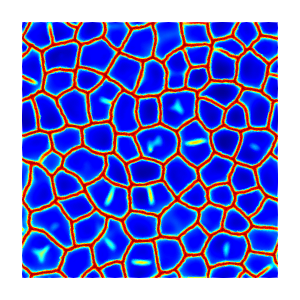
\includegraphics[width=\textwidth]{Appendices/figures/damage.png}
    \caption{}
  \end{subfigure}
  \begin{subfigure}[b]{0.36\textwidth}
    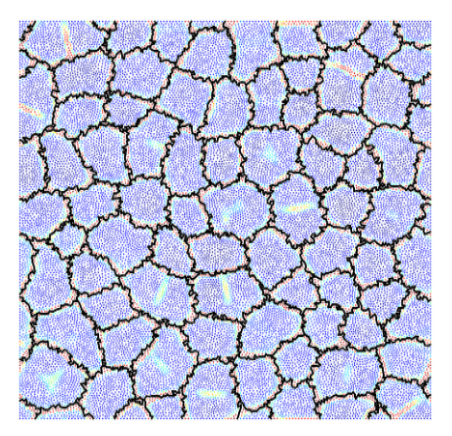
\includegraphics[width=\textwidth]{Appendices/figures/cluster.png}
    \vspace{-0.06in}
    \caption{}
  \end{subfigure}
  \caption{ (a) Final phase field obtained using a spatially correlated random $\Gc$ and $\psi_c$. (b) Corresponding clusters labeled by the flooding algorithm. Cluster boundaries are marked in black. }
  \label{fig: clustering}
\end{figure}

The algorithm has a fundamental ``flooding'' structure.  In particular, a seeding element broadcasts its information to all of its geometric neighbors, and each neighbor becomes a new seed for the next round of information propagation. In the context of counting fragments, the information of an element includes its state and the cluster it belongs to. An element is considered to be ``intact'' if all of its nodal damage values are below $d_{\text{th}}$, otherwise it is considered to be ``broken''.

Three lists are managed by the algorithm. The first list \texttt{ALL} includes all elements that need to be classified. The second list \texttt{CANDIDATE}, optionally a first-in-first-out (FIFO) queue, includes all candidate elements for the current cluster. The third list \texttt{BROKEN} includes all ``broken'' elements. Each cluster $\texttt{CLUSTER}^i$ is essentially a list of elements that belong to the same parent cluster.

The algorithm consists of three stages. In the first stage, we update the damage values of all nodes and states of all elements. All elements that have a status change require reclassification. Therefore, any cluster that contains elements pending reclassification is pushed into \texttt{ALL} for future reclassification.

In the second stage, all ``intact'' elements in \texttt{ALL} are pushed into \texttt{CANDIDATE} one at a time until \texttt{ALL} has no more ``intact'' elements. Each new cluster is constructed by dequeueing \texttt{CANDIDATE}. The first element in \texttt{CANDIDATE} is dequeued after all of its connecting ``intact'' elements from \texttt{ALL} are pushed into \texttt{CANDIDATE}.

During the third stage, ``broken'' elements are grouped into their nearest cluster to preserve the total volume of the mesh. In our implementation,  ``broken'' elements are assigned to clusters based on the solution to a minimization problem of weighted Euclidean distance between the elements and cluster centroids.

\begin{algorithm}[!htb]
  \setstretch{1.2}
  \caption{An iterative flooding algorithm for fragmentation count}
  \begin{algorithmic}[1]
    \State Set $d_0 \leftarrow 0$
    \State Set cluster count $c \leftarrow 0$
    \State Group all elements into $\texttt{CLUSTER}^c$
    \For {time step $n \in \{0, 1, 2,...\}$}
    \For {each cluster $\texttt{CLUSTER}^i$}
    \State Move all ``broken'' elements into \texttt{BROKEN}
    \If {$\texttt{CLUSTER}^i$ contains any element that has a state change, i.e.\ from ``intact'' to ``broken'' }
    \State {Move all remaining elements into \texttt{ALL}}
    \EndIf
    \EndFor
    \While {\texttt{ALL} is not empty}
    \If {All elements in \texttt{ALL} are ``broken''}
    \State {Move all elements in \texttt{ALL} into \texttt{BROKEN}}
    \State {Break while loop}
    \Else
    \State {Move one ``intact'' element from \texttt{ALL} to \texttt{CANDIDATE}}
    \State {Increment cluster count $c \leftarrow c+1$}
    \While{\texttt{ALL} is not empty}
    \For {each element $e$ that shares a common edge with the first element in the queue \texttt{CANDIDATE}}
    \If {$e$ is ``intact''}
    \State {Enqueue $e$ into \texttt{CANDIDATE}}
    \Else
    \State {Move $e$ into \texttt{BROKEN}}
    \EndIf
    \EndFor
    \State {Dequeue first element in \texttt{CANDIDATE} into $\texttt{CLUSTER}^c$}
    \EndWhile
    \EndIf
    \EndWhile
    \State {Move all elements in \texttt{BROKEN} into their nearest cluster}
    \EndFor
  \end{algorithmic}
  \label{alg: flooding}
\end{algorithm}

The skeleton of the flooding algorithm is outlined in Algorithm \ref{alg: flooding}.

\begin{figure}[htb!]
  \centering
  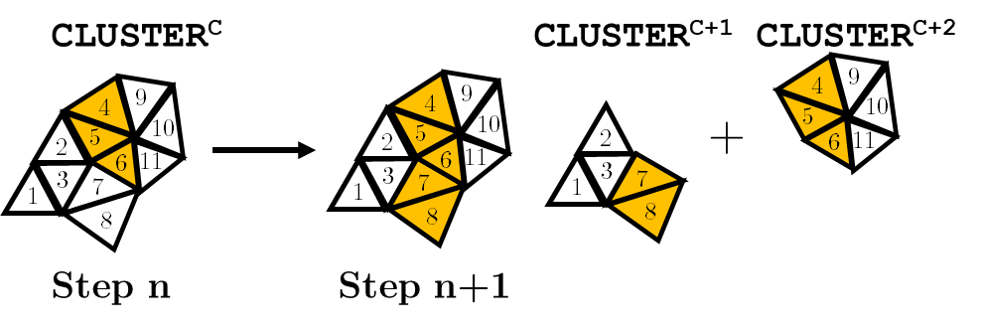
\includegraphics[width=0.75\textwidth]{Appendices/figures/status_change.png}
  \caption{Status change from step n to step n+1. ``Broken'' elements are labeled in yellow, and ``intact'' elements are white. The step-by-step reclassification procedure is shown in Table \ref{tab: flooding demo}.}
  \label{fig: flooding demo}
\end{figure}

\begin{table}[htbp!]
  \scriptsize
  \centering
  \caption{Demonstration of classification after the update from time step n to time step n+1. Broken elements are denoted with an underscore.}
  \begin{tabular}{r c c c c | l}
    \toprule
    Step & Stage & \texttt{ALL}        & \texttt{CANDIDATE} & \texttt{BROKEN}                                                             & Comments                                                                                                       \\
    \midrule
    n    &       & $\emptyset$         & $\emptyset$        & $\emptyset$                                                                 & $\texttt{CLUSTER}^c = \{1,2,3,\underline{4},\underline{5},\underline{6},7,8,9,10,11\}$                         \\
    n+1  &       & $\emptyset$         & $\emptyset$        & $\emptyset$                                                                 & $\texttt{CLUSTER}^c = \{1,2,3,\underline{4},\underline{5},\underline{6},\underline{7},\underline{8},9,10,11\}$ \\
    n+1  & 1     & $\{1,2,3,9,10,11\}$ & $\emptyset$        & $\{\underline{4},\underline{5},\underline{6},\underline{7},\underline{8}\}$ & Declassify $\texttt{CLUSTER}^c$                                                                                \\
    n+1  & 2     & $\{2,3,9,10,11\}$   & $\{1\}$            & $\{\underline{4},\underline{5},\underline{6},\underline{7},\underline{8}\}$ & Enqueue element 1 to \texttt{CANDIDATE}                                                                        \\
    n+1  & 2     & $\{9,10,11\}$       & $\{1,2,3\}$        & $\{\underline{4},\underline{5},\underline{6},\underline{7},\underline{8}\}$ & Enqueue connected elements 2, 3                                                                                \\
    n+1  & 2     & $\{9,10,11\}$       & $\{2,3\}$          & $\{\underline{4},\underline{5},\underline{6},\underline{7},\underline{8}\}$ & Dequeue element 1                                                                                              \\
    n+1  & 2     & $\{9,10,11\}$       & $\{3\}$            & $\{\underline{4},\underline{5},\underline{6},\underline{7},\underline{8}\}$ & Dequeue element 2                                                                                              \\
    n+1  & 2     & $\{9,10,11\}$       & $\emptyset$        & $\{\underline{4},\underline{5},\underline{6},\underline{7},\underline{8}\}$ & Dequeue element 3                                                                                              \\
         &       &                     &                    &                                                                             & $\texttt{CLUSTER}^{c+1} = \{1,2,3\}$                                                                           \\
    n+1  & 2     & $\{10,11\}$         & $\{9\}$            & $\{\underline{4},\underline{5},\underline{6},\underline{7},\underline{8}\}$ & Enqueue element 9 to \texttt{CANDIDATE}                                                                        \\
    n+1  & 2     & $\emptyset$         & $\{9,10,11\}$      & $\{\underline{4},\underline{5},\underline{6},\underline{7},\underline{8}\}$ & Enqueue connected elements 10, 11                                                                              \\
    n+1  & 2     & $\emptyset$         & $\{10,11\}$        & $\{\underline{4},\underline{5},\underline{6},\underline{7},\underline{8}\}$ & Dequeue element 9                                                                                              \\
    n+1  & 2     & $\emptyset$         & $\{11\}$           & $\{\underline{4},\underline{5},\underline{6},\underline{7},\underline{8}\}$ & Dequeue element 10                                                                                             \\
    n+1  & 2     & $\emptyset$         & $\emptyset$        & $\{\underline{4},\underline{5},\underline{6},\underline{7},\underline{8}\}$ & Dequeue element 11                                                                                             \\
    n+1  & 3     & $\emptyset$         & $\emptyset$        & $\{\underline{4},\underline{5},\underline{6}\}$                             & Group elements 7, 8 into $\texttt{CLUSTER}^{c+1}$                                                              \\
    n+1  & 3     & $\emptyset$         & $\emptyset$        & $\emptyset$                                                                 & Group elements 4, 5, 6 into $\texttt{CLUSTER}^{c+2}$                                                           \\
    \bottomrule
  \end{tabular}
  \label{tab: flooding demo}
\end{table}
